%; whizzy chapter
% -initex iniptex -latex platex -format platex -bibtex jbibtex -fmt fmt
% 以上 whizzytex を使用する場合の設定。

%     Kansai Debian Meeting resources
%     Copyright (C) 2007 Takaya Yamashita
%     Thank you for Tokyo Debian Meeting resources

%     This program is free software; you can redistribute it and/or modify
%     it under the terms of the GNU General Public License as published by
%     the Free Software Foundation; either version 2 of the License, or
%     (at your option) any later version.

%     This program is distributed in the hope that it will be useful,
%     but WITHOUT ANY WARRANTY; without even the implied warranty of
%     MERCHANTABILITY or FITNESS FOR A PARTICULAR PURPOSE.  See the
%     GNU General Public License for more details.

%     You should have received a copy of the GNU General Public License
%     along with this program; if not, write to the Free Software
%     Foundation, Inc., 51 Franklin St, Fifth Floor, Boston, MA  02110-1301 USA

%  preview (shell-command (concat "evince " (replace-regexp-in-string "tex$" "pdf"(buffer-file-name)) "&"))
% 画像ファイルを処理するためにはebbを利用してboundingboxを作成。
%(shell-command "cd image200708; ebb *.png")

%%ここからヘッダ開始。

\documentclass[mingoth,a4paper]{jsarticle}
\usepackage{kansaimonthlyreport}
\usepackage[dvips]{xy}
\usepackage{ulem}

% 日付を定義する、毎月変わります。
\newcommand{\debmtgyear}{2013}
\newcommand{\debmtgdate}{22}
\newcommand{\debmtgmonth}{12}
\newcommand{\debmtgnumber}{79}

\def\fixme#1{{\color{red}{#1}}}

\begin{document}

\begin{titlepage}

% 毎月変更する部分、本文の末尾も修正することをわすれずに

 第\debmtgnumber{}回 関西 Debian 勉強会資料

\vspace{2cm}

\begin{center}
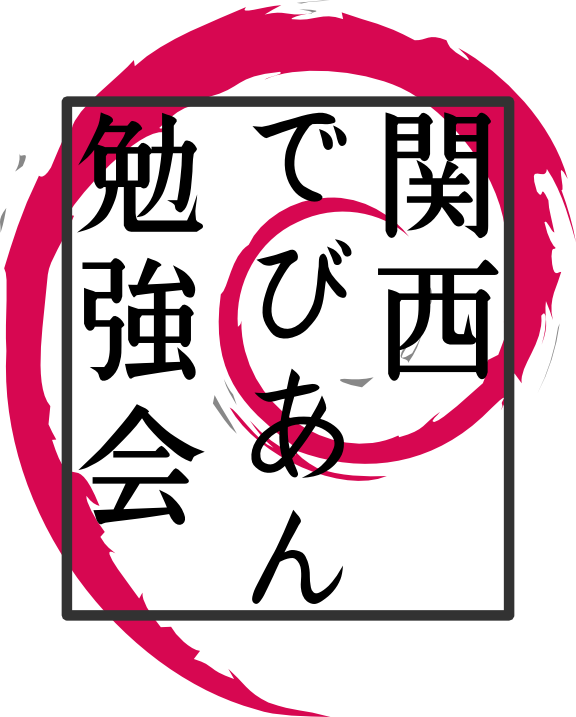
\includegraphics{image200802/kansaidebianlogo.png}
\end{center}

\begin{flushright}
\hfill{}関西 Debian 勉強会担当者 佐々木・倉敷・のがた・かわだ・八津尾 \\
\hfill{}\debmtgyear{}年\debmtgmonth{}月\debmtgdate{}日
\end{flushright}

\thispagestyle{empty}
\end{titlepage}

\dancersection{Introduction}{Debian JP}

\vspace{1em}

 関西Debian勉強会はDebian GNU/Linuxのさまざまなトピック
 (新しいパッケージ、Debian特有の機能の仕組、Debian界隈で起こった出来事、
 などなど)について話し合う会です。

 目的として次の三つを考えています。
 \begin{itemize}
  \item MLや掲示板ではなく、直接顔を合わせる事での情報交換の促進
  \item 定期的に集まれる場所
  \item 資料の作成
 \end{itemize}

 それでは、楽しい一時をお過ごしください。

\newpage

\begin{minipage}[b]{0.2\hsize}
 {\rotatebox{90}{\fontsize{80}{80}
{\gt 関西 Debian 勉強会}}}
\end{minipage}
\begin{minipage}[b]{0.8\hsize}
\hrule
\vspace{2mm}
\hrule
\setcounter{tocdepth}{1}
\tableofcontents
\vspace{2mm}
\hrule
\end{minipage}

\dancersection{最近のDebian関係のイベント報告}{Debian JP}

\subsection{第77回関西Debian勉強会}

77回目の関西Debian勉強会は10月27日(日)に、港区民センターで行なわれまし
た。

セッションは坂本さんによる「ALSAのユーザランド解説」と佐々木さんによる
「git-buildpackage入門again」の二本でした。

9月の勉強会に続いて坂本さんにサウンドの話題、今回はALSAのユーザランドを
解説していただきました。事前課題でプログラムをコンパイルしてくるのは初
でしたが、みなさんなんなく課題をこなしてきていただけたようです。
(結果は思ったように収束していないようでしたが。)

git-buildpackage入門では、各自が気になっていたパッケージをgit-buildpackage
を使ってパッケージ化する実演を行ないながら、各コマンドを掘り下げていき
ました。gbpで呼びだすようになっていたり、便利な新しいコマンドが追加さ
れていたりと、以前の入門時よりいろいろと変わっていました。

\subsection{第78回関西Debian勉強会@関西オープンソース2013}
78回目の関西Debian勉強会は11月9日(土)に、大阪南港ATCで行なわれた関西
オープンソース2013に出張開催という形で行なわれました。

当日は、セッションとブース展示を行ないました。
セッションは「Debian7.0の実情/今後の開発について」と題して佐々木さんが
行ない、朝早くからの開催でしたが約20名の方に参加していただきました。
またブースでは、Raspberry Pi、MK802の実機展示とあんどきゅめんてぃっど
でびあん最新号の販売などを行ないました。

\subsection{第106,107回東京エリアDebian勉強会}

106回目の東京エリアDebian勉強会は11月16日(土)にあんさんぶる荻窪で行な
われました。

セッションは野島さんの「waylandを動かす」と上川さんの「Emacs tramp(transparent remote file access)」
の二本でした。

107回目の東京エリアDebian勉強会は12月21日(土)にあんさんぶる荻窪で行な
われました。

セッションは野島さんの「debian GNU/Hurd」と「Debian勉強会2014年度計画」の二本でした。

みんな、EmacsとかHurdとか好きですよね。

\subsection{第0,1回Debianもくもくの会}
Debianもくもくの会が11月23日(土)にミラクル・リナックスさんで、
12月14日(土)には朝日ネットさんで開催されました。

今年のバグは今年のうちにということでみなさんもくもくと作業されていたよ
うで、タイムライン\#debmokuも静かでした。

\subsection{Debian Project}
\subsubsection{Debian Policy 3.9.5.0 released}
10月28日にDebian Policyが改訂され3.9.5.0がリリースされました。
\footnote{\url{http://lists.debian.org/debian-devel-announce/2013/10/msg00006.html}}

主な変更は、「パッケージはアップグレード中にローカルな変更が加えられていない廃止
された設定ファイルを削除するべきである」(10.7.3)です。他にも11の変更点があります。

このリリースをもって、長らくDebian Policyの編集者であった、Charles Plessyさんが
辞められました。おつかれさまでした。
さすがにポリシーを扱うとなると他のパッケージの面倒をみていられるほどの余裕はなく
なるようです。

\subsubsection{Alioth is down/alioth back online}

DebianプロジェクトのソフトウェアをホスティングしているAlioth.debian.orgが11月10日
ごろに落ちました。
\footnote{\url{http://lists.debian.org/debian-infrastructure-announce/2013/11/msg00001.html}}
ディスク障害だったようですが、リビルド処理中に再度別のディスク障害が発生し復旧が
長引いたようです。
\footnote{\url{http://lists.debian.org/debian-infrastructure-announce/2013/11/msg00002.html}}

この勉強会資料のリポジトリもAliothでホスティングしているのでその間資料の更新がで
きなくなりました。ちょうど東京エリアDebian勉強開催準備中で、告知ページはどうしよ
うもなかったようですが、資料の更新は一時的にgithubに退避するなどして難を逃がれた
ようです。分散型バージョン管理システムって便利ですね。

\subsubsection{Release sprint results - team changes, auto-rm and arch status}
Jessieに向けての作業も着々と進んでいます。\footnote{\url{http://lists.debian.org/debian-devel-announce/2013/11/msg00007.html}}

testingからのAUTOREMOVALSが始まりました。これによって素早いバグ対処、品質向上を
見込まれていますが、今後どのようになっていくか注目です。

サポートアーキテクチャとしてはs390がすでに除外されることが決まっています
\footnote{\url{http://lists.debian.org/debian-devel-announce/2013/10/msg00005.html}}
が、ia64も除外対象となりそうです。
HurdもJessieではリリース対象とならないであろうと見込まれています。

また、アートワークの募集も始まっています
\footnote{\url{http://lists.debian.org/debian-devel-announce/2013/11/msg00002.html}}
今度はどんな感じになるのか今から楽しみです。

\dancersection{事前課題}{Debian JP}

今回の課題は以下の通りです。
\begin{screen}
  \begin{enumerate}
  \item %
    Debian 界隈で今年印象に残っていること、話題を教えてください。
  \end{enumerate}
\end{screen}

参加者の皆さんの解答は以下の通りです:

\begin{prework}{ かわだてつたろう }
  \begin{enumerate}
  \item wheezy リリースかな

    ちょこっとレシピに記事も書かせてもらいました。
  \end{enumerate}
\end{prework}

\begin{prework}{ 川江 }
  \begin{enumerate}
  \item Wheezyのリリースかな?
  \end{enumerate}
\end{prework}

\begin{prework}{ 佐々木洋平 }
  \begin{enumerate}
  \item
    \begin{itemize}
    \item Wheezy がリリースされた事
    \item 大統一Debian勉強会
    \end{itemize}

    かな。月並ですが。
  \end{enumerate}
\end{prework}

\begin{prework}{ 木下 }
  \begin{enumerate}
  \item Debian 7.0 Wheezyのリリース

    →メジャーなアーキテクチャだけでなく、個人的ですが、PandaBoard等評価キットのポーティングも行われ、実際に手にすることができましたので、驚きと嬉しさで一杯です。それらを実現してくださった方々に感謝致します。
  \end{enumerate}
\end{prework}

\begin{prework}{ 山城の国の住人 久保博 }
  \begin{enumerate}
  \item
    \begin{itemize}
    \item Wheezy のリリース
    \item 道場で勉強した quilt の仕組み
    \item Software Design 誌での Debian Hot Topics の連載
    \end{itemize}
  \end{enumerate}
\end{prework}

\begin{prework}{ lurdan }
  \begin{enumerate}
  \item 無事に Wheezy がリリースされたなぁとか SteamOS が Debian ベースだったとか
  \item 状況もかわってきてるし、ちっと運営方法を変えてみるのもいいかもねー
  \end{enumerate}
\end{prework}

\dancersection{2013年の振り返りと2014年の企画}{Debian JP}

2013年も今月で最後の関西Debian勉強会になります。
2007年3月からはじまった勉強会も今年で7年目になり、来年には80回目を迎えようとしています。
昨年に続いて「大統一Debian勉強会」を開催することもできました。継続してイベント開催が行なえたことは収穫だと思っています。

\subsection{勉強会全体について}

\subsubsection{月刊Debian Policy}

昨年から始めた「月刊 Debian Policy」ですが、今年は1回しか進めることができませんでした。
10月にDebian Policy Manual
\footnote{
  \url{http://www.debian.org/doc/debian-policy/}\newline
  現時点での最新版は 3.9.5.0, 2013-10-28
}
が改訂されましたので、これを機に再開して今後も進めて行きたいと思います。

\subsubsection{GNOMEネタ}

今年5月にリリースされたWheezyからGNOME3になりました。GNOME3は今までのGNOME2とは大
きく変わっています。
Debianの標準デスクトップ環境でもあるGNOMEがどうなっているのかということで、3月には
GNOMEについての発表が行なわれました。
GNOMEの変化は各所で話題になっており、debian-devel@d.o 上でもsystemdとの関連や標準
デスクトップをGNOMEから別のもの(xfce)に変更するなど盛り上がっています。
勉強会でも今後の変化について追いかけていきたいですね。

\subsubsection{その他, 定例ネタ}

毎回のセッションについてですが、
今年は「Using Drupal on Debian」でDrupalプロジェクトの紀野さん、「Debian Installer
トラブルシューティング」でGREEのYuryuさん、Ubuntu Japanese Teamからいくやさん、坂
本さん、GNOMEネタの回には、直前で都合がつかなくなってしまいましたが、GNOMEプロジェ
クトの松澤さんといった他のコミュニティの方々を招いて発表していただきました。

今年は「リリースノートを読んでみよう。」「Debianの歩き方」「git-buildpackage」と
いわゆる定番のネタが少なかった気がします。
来年は定番のネタ(Debianの入門的なお話、ライセンス、パッケージ作成、BTS)などの題材
を定期的にできたら良いかなと考えています。

\subsection{運営}

運営に関しては、毎月の継続した開催は行なってきていました。
事前の準備、告知が不十分な場合もありましたので、今後はもう少し個人の負担を減らし
つつ改善していきたいと考えています。

\subsection{イベント/NM申請}

イベント参加については、OSC Kansai@Kyoto、KOF2013に参加しました。
勉強会からforkしたGPGキーサインパーティも毎回実施されています。今後も継続して参加
する予定です。
%
また、昨年のような合宿イベントは開催できませんでしたが、6月には東京エリアDebian
勉強会と福岡Debian勉強会と合同で「大統一Debian勉強会」を日本大学で開催しました。
これらのイベントは今後も継続して実施する予定です。

Debian開発者への道、として昨年から佐々木さんと倉敷さんの二人がNMプロセスの申請を
進められています。
今後もNMプロセスに挑む参加者やDebian Maintainerとなって精力的にパッケージを開発/
更新する人が増えると良いですね。

\subsection{開催実績}

関西Debian勉強会の出席状況を確認してみましょう。グラフで見る
と\fgref{fig:kansaipeoplechart}になります。また、毎回の参加者、アンケート
回答者の人数とその際のトピックを \tbref{tab:count2013kansai} にまとめまし
た。グラフ中の黒線は参加人数、赤線は1年の移動平均、青線はアンケートの回答
人数です。参加人数が$0$となっているところは人数が集計されていないor開催さ
れなかった月です。アンケートの回答人数が$0$となっているところはアンケート
が実施されなかった月です。

Debian勉強会申し込みシステムを使用することで、事前課題は毎回設定するようになり
ましたが、アンケートシステムは毎回設定するまで活用できませんでした。
%
\begin{figure}[h]
  \begin{center}
    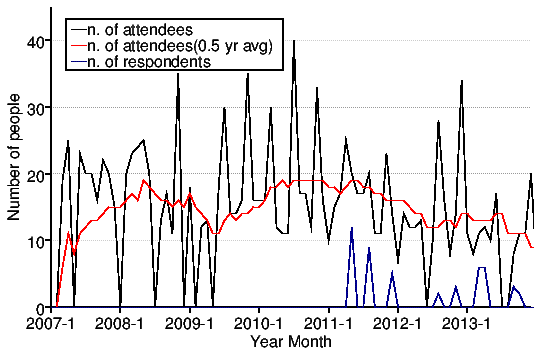
\includegraphics[width=.6\hsize]{image201312/memberanalysis/kansai.png}
  \end{center}
  \caption{関西の参加人数推移(参加人数と6ヶ月移動平均、アンケート回答人数)}
  \label{fig:kansaipeoplechart}
\end{figure}

%\pagebreak

\begin{table}
  \begin{minipage}{.5\linewidth}
  \caption{関西Debian勉強会の参加人数とトピック(2007-2008年)}
  \begin{center}
    \begin{tabular}{|l|c|p{10em}|}
      \hline
                 & 参加人数 & 内容 \\
      \hline
      2007年3月  & 19       & 開催にあたり \\
      2007年4月  & 25       & goodbye、youtube、プロジェクトトラッカー\\
      2007年6月  & 23       & 社会契約、テーマ、debian/rules、bugreport\\
      2007年7月  & 20前後   & OSC-Kansai \\
      2007年8月  & 20       & Inkscape、patch、dpatch\\
      2007年9月  & 16       & ライブラリ、翻訳、debtorrent\\
      2007年10月 & 22       & 日本語入力、SPAMフィルタ\\
      2007年11月 & 20前後   & KOF \\
      2007年12月 & 15       & 忘年会、iPod touch\\
      \hline
      \hline
                 & 参加人数 & 内容 \\
      \hline
      2008年2月  & 20       & PC Cluster, GIS, \TeX \\
      2008年3月  & 23       & bug report, developer corner, GPG \\
      2008年4月  & 24       & coLinux, Debian GNU/kFreeBSD, sid \\
      2008年5月  & 25       & ipv6, emacs, ustream.tv\\
      2008年6月  & 20       & pbuilder, hotplug, ssl\\
      2008年8月  & 13       & coLinux \\
      2008年9月  & 17       & debian mentors, ubiquity, DFSG\\
      2008年10月 & 11       & cdbs,cdn.debian.or.jp \\
      2008年11月 & 35       & KOF \\
      2008年12月 & ?        & TeX資料作成ハンズオン\\
      \hline
    \end{tabular}
  \end{center}
\end{minipage}
\pagebreak
\begin{minipage}{.5\linewidth}
  \begin{center}
    \caption{関西Debian勉強会の参加人数とトピック(2009-2010)}
    \begin{tabular}{|l|c|p{10em}|}
      \hline
                 & 参加人数 & 内容 \\
      \hline
      2009年1月  & 18       & DMCK, LT \\
      2009年3月  & 12       & Git \\
      2009年4月  & 13       & Installing sid, Mancoosi, keysign \\
      2009年6月  & 18       & Debian Live, bash\\
      2009年7月  & 30?      & OSC2009Kansai \\
      2009年8月  & 14       & DDTSS, lintian \\
      2009年9月  & 14       & reportbug, debian mentors\\
      2009年10月 & 16       & gdb, packaging \\
      2009年11月 & 35       & KOF2009 \\
      2009年12月 & 16       & GPS program, OpenStreetMap \\
      \hline
      \hline
                 & 参加人数 & 内容 \\
      \hline
      2010年1月  & 16       & Xen, 2010年企画 \\
      2010年2月  & 16       & レンタルサーバでの利用, GAE \\
      2010年3月  & 30?      & OSC2010Kobe \\
      2010年4月  & 12       & デスクトップ環境, 正規表現 \\
      2010年5月  & 11       & ubuntu, squeeze \\
      2010年6月  & 11       & debhelper7, cdbs, puppet \\
      2010年7月  & 40?      & OSC2010Kyoto \\
      2010年8月  & 17       & emdebian, kFreeBSD \\
      2010年9月  & 17       & タイルWM \\
      2010年10月 & 12       & initramfs, debian live \\
      2010年11月 & 33       & KOF2010 \\
      2010年12月 & 14       & Proxmox, annual review \\
      \hline
    \end{tabular}
  \end{center}
\end{minipage}
\end{table}
\pagebreak
\begin{table}
%  \begin{minipage}{.5\linewidth}
    \caption{関西Debian勉強会の参加人数とトピック(2011)}
    \begin{center}
      %\begin{tabular}{|l|c|c|p{10em}|}
      \begin{tabular}{|l|c|c|l|}
        \hline
        開催年月  & 参加人数 & 回答人数 & 内容 \\
        \hline
        2011年1月 &10        & 0        & BTS, Debian GNU/kFreeBSD\\
        2011年2月 &15        & 0        & pbuilder, Squeezeリリースパーティ\\
        2011年3月 &17        & 0        & ライセンス, Debianのドキュメント関連\\
        2011年4月 &25        & 0        & OSC 2011 Kansai @ Kobe, GPG キーサインパーティ \\
        2011年5月 &20        &12        & vi, dpkg \\
        2011年6月 &17        & 0        & IPv6, vcs-buildpackage{svn, git}\\
        2011年7月 &17        & 0        & OSC 2011 Kansai @ Kyoto, GPG キーサインパーティ\\
        2011年8月 &20        & 9        & Debianパッケージ作成ハンズオン\\
        2011年9月 &11        & 0        & vcs-buildpackage{bzr, git}\\
        2011年10月&11        & 0        & Emacs, vim の拡張のDebianパッケージ, 翻訳\\
        2011年11月&23        & 0        & KOF 2011\\
        2011年12月&13        & 5        & NMプロセス, BTS\\
        \hline
      \end{tabular}
    \end{center}
%  \end{minipage}
%  \begin{minipage}{.5\linewidth}
    \caption{関西Debian勉強会の参加人数とトピック(2012)}
    \label{tab:count2012kansai}
    \begin{center}
%      \begin{tabular}{|l|c|c|p{10em}|}
      \begin{tabular}{|l|c|c|l|}
        \hline
        開催年月  & 参加人数 & 回答人数 & 内容 \\
        \hline
        2012年1月 & 7        &0         & Debian温泉合宿 \\
        2012年2月 &14        &0         & autofs+pam\_chroot, t-codeその1, 月刊Debian Policy その1 \\
        2012年3月 &12        &0         & 新年度スケジューリング, Konohaその1, t-codeその2, 月刊Debian Policy その2 \\
        2012年4月 &12        &0         & フリーソフトウェアと著作権, Konohaその2, 月刊Debian Policy その3 \\
        2012年5月 &13        &0         & DebianとLDAP(頓挫), ITP入門, 月刊Debian Policy その4 \\
        2012年6月 & -        &0         & 大統一Debian勉強会 \\
        2012年7月 &10        &0         & DebianとLDAPその1, 大統一Debian勉強会報告, 月刊Debian Policy その5 \\
        2012年8月 &28        &2         & OSC 2012 Kansai @ Kyoto, GPG キーサインパーティ\\
        2012年8月 &16        &0         & DebianとKerberos, News from EDOS \\
        2012年9月 & 8        &0         & clang によるパッケージビルド, 月刊Debian Policy その6 \\
        2012年10月&14        &3         & 翻訳環境構築, DSAの舞台裏\\
        2012年11月&34        &0         & KOF 2012\\
        2012年12月&12        &0         & Debian on Android, 月刊Debian Policy その7 \\
        \hline
      \end{tabular}
    \end{center}
%  \end{minipage}
\end{table}
\pagebreak
\begin{table}
    \caption{関西Debian勉強会の参加人数とトピック(2013)}
    \label{tab:count2013kansai}
    \begin{center}
%      \begin{tabular}{|l|c|c|p{10em}|}
      \begin{tabular}{|l|c|c|l|}
        \hline
        開催年月  & 参加人数 & 回答人数 & 内容 \\
        \hline
        2013年1月 & 8        &0         & Using Drupal on Debian, 月刊Debian Policy その8 \\
        2013年2月 &11        &6         & Debian Installerトラブルシューティング, Ruby In Wheezy \\
        2013年3月 &12        &6         & UbuntuとGNOME Shellと私, 管理者視点からのGNOMEの大規模な配置 \\
        2013年4月 &10        &0         & リリースノートを読んでみよう。, \\
                  &          &          & クラウド初心者がAWSにDebianをのっけて翻訳サービスの試行に挑戦してみた \\
        2013年5月 &17        &0         & DebianとUbuntuの違いを知ろう, Debianの歩き方 \\
        2013年6月 & -        &0         & 大統一Debian勉強会 \\
        2013年7月 &          &0         & OSC 2013 Kansai @ Kyoto, GPG キーサインパーティ\\
        2013年8月 & 8        &3         & puppetによる構成管理の実践 \\
        2013年9月 &11        &2         & Linuxとサウンドシステム, dgitでソースパッケージを触ってみる \\
        2013年10月&11        &0         & ALSAのユーザーランド解説, git-buildpackage入門again \\
        2013年11月&20        &0         & KOF 2013 \\
        2013年12月& 6        &0         & 2013年の振り返りと2014年の企画, 忘年会 \\
        \hline
      \end{tabular}
    \end{center}
\end{table}

\clearpage

\dancersection{今後の予定}{Debian JP}

\subsection{関西Debian勉強会}

次回、第80回関西Debian勉強会は1月26日(日)に開催します。

内容はこのときには決まっているはず。

\subsection{東京エリアDebian勉強会}
第108回東京エリアDebian勉強会は内容、会場などはまだ未定ですが1月に開催
予定です。

%
% 冊子にするために、4の倍数にする必要がある。
% そのための調整
\dancersection{メモ}{}
\mbox{}\newpage
\mbox{}\newpage
%% \mbox{}\newpage

\printindex
%\cleartooddpage

 \begin{minipage}[b]{0.2\hsize}
  \rotatebox{90}{\fontsize{80}{80} {\gt 関西 Debian 勉強会} }
 \end{minipage}
 \begin{minipage}[b]{0.8\hsize}

 \vspace*{15cm}
 \rule{\hsize}{1mm}
 \vspace{2mm}
 
\includegraphics[width=2cm]{image200502/openlogo-nd.eps}
 \noindent \Large \bfseries{Debian 勉強会資料}\\ \\
 \noindent \normalfont \debmtgyear{}年\debmtgmonth{}月\debmtgdate{}日 \hspace{5mm}  初版第1刷発行\\
 \noindent \normalfont 関西 Debian 勉強会 (編集・印刷・発行)\\
 \rule{\hsize}{1mm}
 \end{minipage}

\end{document}
